\subsection{Hardware Setup}
Der Raspberry Pi muss mit seiner Stromversorgung (USB C), einem  Netzwerk (Ethernet) und 1-12 Sensorboards verbunden werden.
\subsection{Messung Starten}
Über das Terminal (Unter Windows cmd) muss eine SSH Verbindung zum Raspberry Pi aufgebaut werden.\\
\textbf{ssh pi@[IP-ADRESSE]}\\
Die Messsoftware befindet sich im Ordner $\sim$/SpectralSensor\\
\textbf{cd  $\sim$/SpectralSensor}\\
Damit die Messsoftware auch noch weiter läuft, wenn die SSH Verbindung wieder geschlossen wird, muss sie in einem Screen kompiliert werden.\\
\textbf{screen}\\
\textbf{make}\\
Um die SSH Verbindung zu trennen, ohne die Messung zu unterbrechen, wird einfach das Terminal/CMD Fenster geschlossen.\smallskip

\begin{figure}[H]
\centering
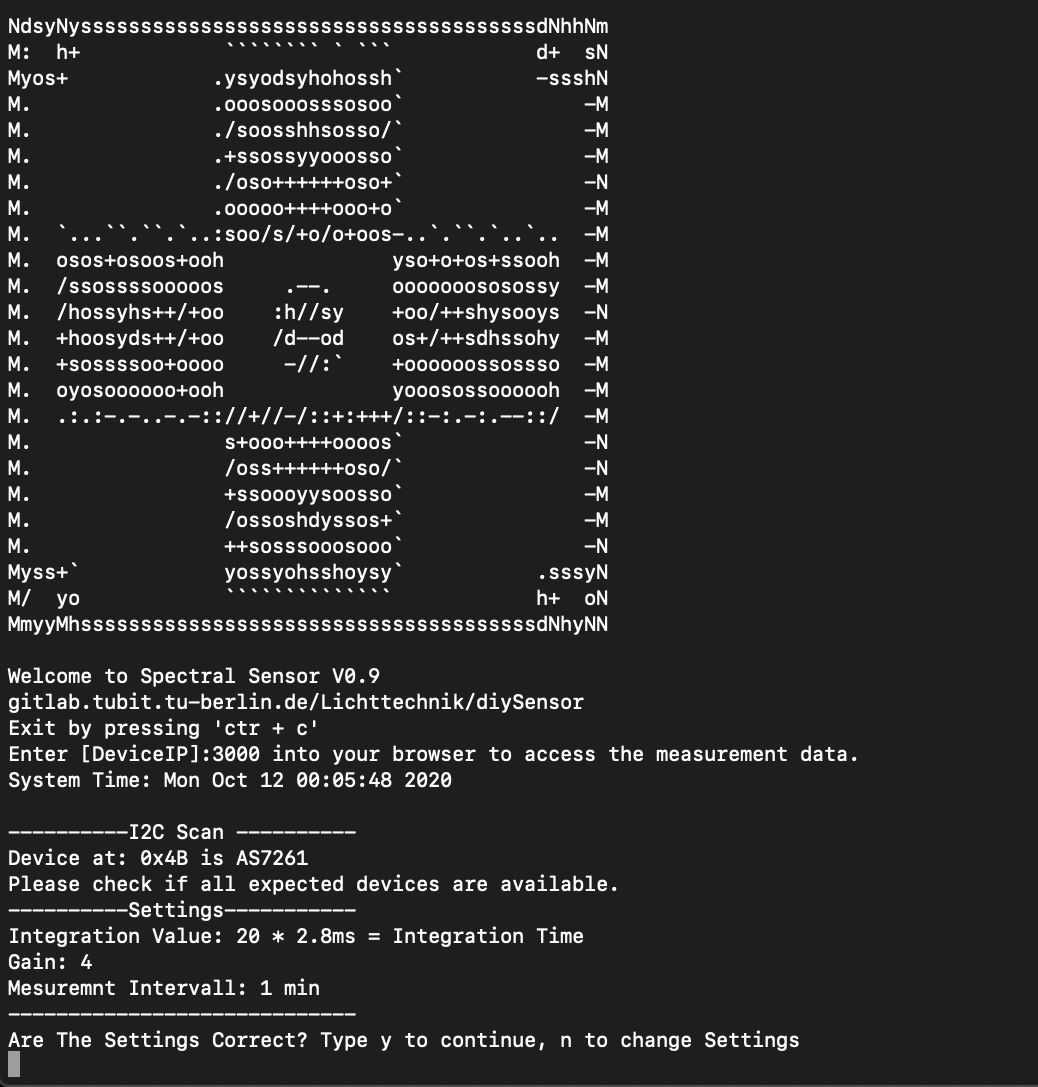
\includegraphics[width=0.7\textwidth]{img/handbuch/check_settings}
\caption{Terminal Output bei Start der Messsoftware }
\label{fig:Start-der-Messsoftware}
\end{figure}
\noindent Zuerst muss im Terminaloutput überprüft werden ob der NTP Server synchronisiert ist.
Wird eine falsche Systemzeit, angezeigt muss das Programm nach etwa 40 Sekunden neu Gestartet werden. Anschließend sollte die Systemzeit richtig sein. (Mehr zum Programm Neustart: \ref{restart}).\\
Im I2C Scann sollten alle angeschlossenen Sensoren angezeigt werden.\\
Die Messung wird mit den angezeigten Einstellungen gestartet, indem die Eingabeaufforderung mit \textbf{Y} bestätigt wird.\\
\begin{figure}[H]
\centering
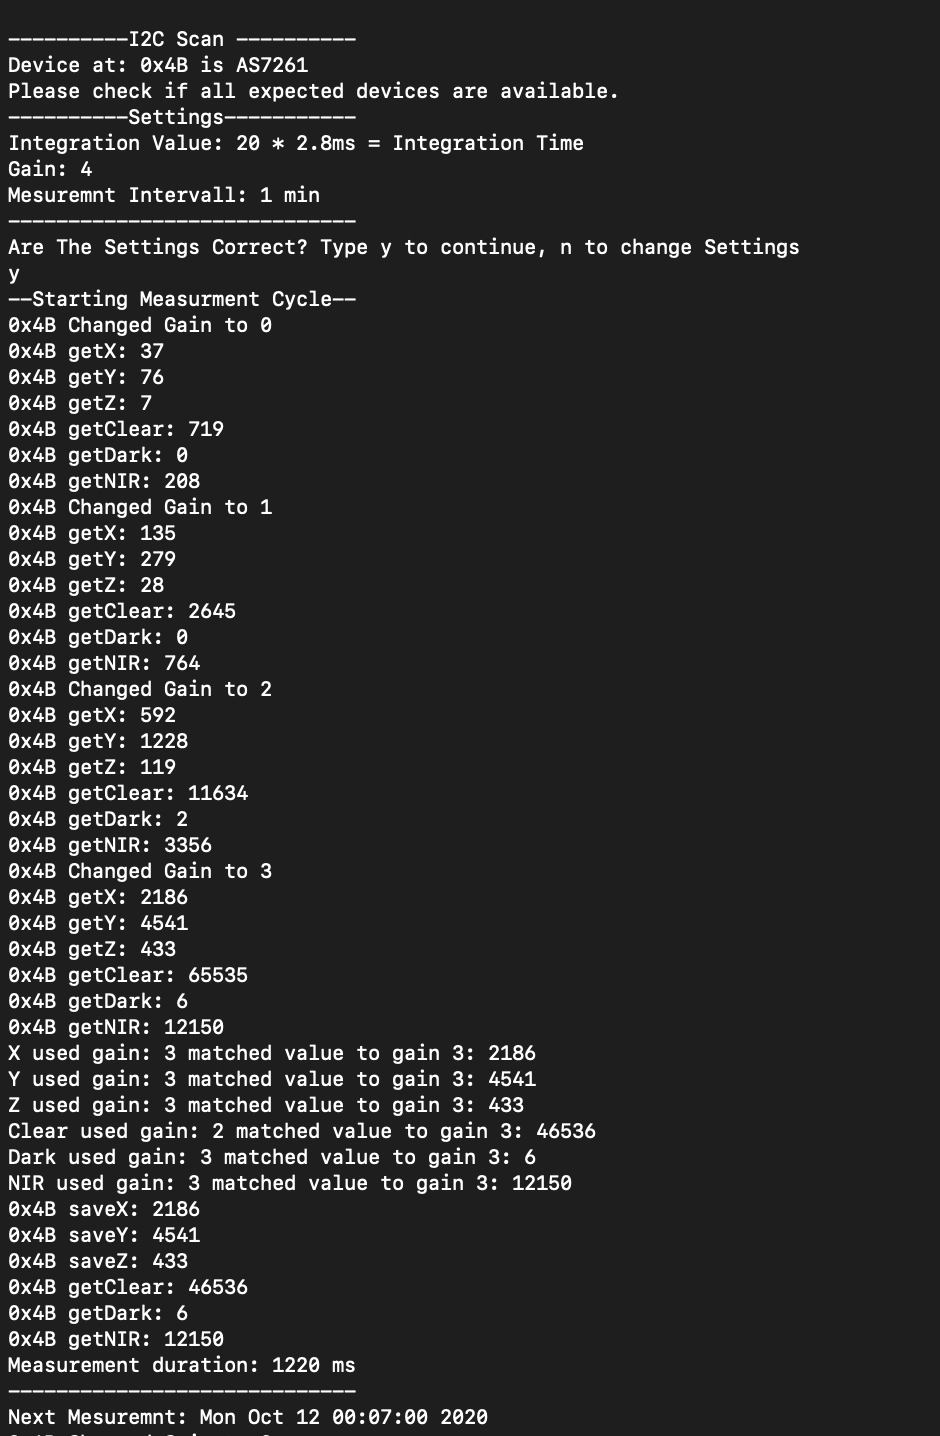
\includegraphics[width=0.7\textwidth]{img/handbuch/y_start_measurement}
\caption{Terminal Output bei Start der Messung }
\label{fig:Start-der-Messung}
\end{figure}

Um die Einstellung zu verändern wird \textbf{N} ausgewählt.\\
\begin{figure}[H]
\centering
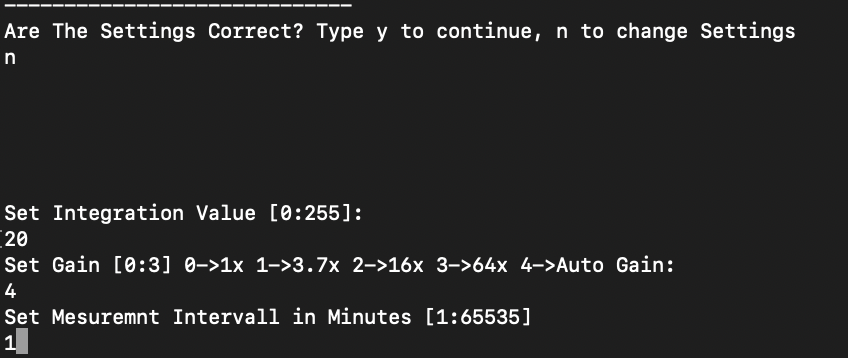
\includegraphics[width=0.7\textwidth]{img/handbuch/n_change_settings}
\caption{Beispielhafter Terminal Output bei Einstellungsänderungen}
\label{fig:changesettings}
\end{figure}
\noindent Die Einstellungen werden nacheinander abgefragt, die Eingaben müssen mit Enter bestätigt werden.\medskip

\noindent Integration Value bestimmt die Integrationszeit, d. h. die Belichtungszeit der einzelnen Messungen.
Gain bestimmt den Verstärkungsfaktor der Messwerte. Im Auto Gain modus wird automatisch der am besten geeigneten Verstärkungsfaktor für jede einzelne Messung ausgewählt.
Measurement Interval ist das Intervall, in dem alle angeschlossenen Sensoren eine Messung durchführen.
\subsection{Einstellung für fortgeschrittene Benutzer}
 \begin{figure}[H]
\centering
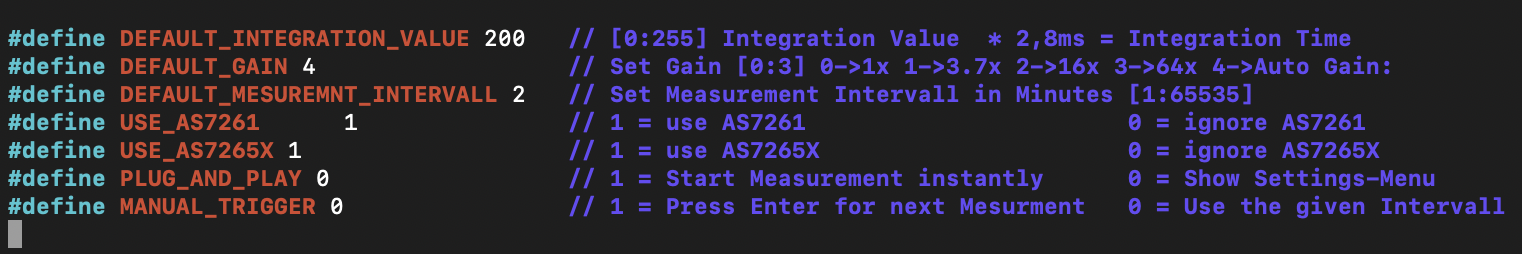
\includegraphics[width=0.9\textwidth]{img/advanced_setting}
\caption{SpectralSensor/defaultvalues.h}
\label{fig:changesettings}
\end{figure}
 In der Datei \textbf{SpectralSensor/defaultvalues.h} können die beim Programmstart vorgeschlagenen Standardeinstellungen angepasst werden.\\
 Zusätzlich kann eingestellt werden, dass die Messung ohne manuelle Benutzerinteraktion direkt mit den Standardeinstellungen startet (PLUG\_AND\_PLAY).\\
 Um die Kalibrierung zu erleichtern, kann der automatische zeitbasierte Auslöser deaktiviert werden (MAUAL\_TRIGGER). Die einzelnen Messungen werden dann durch Drücken der Enter-Taste durchgeführt.
 


\subsection{Webinterface}
Das Grafana Webinterface ist unter folgender Adresse im Browser zu erreichen:\\
\textbf{[IP-ADRESSE]:3000}

\begin{figure}[H]
\centering
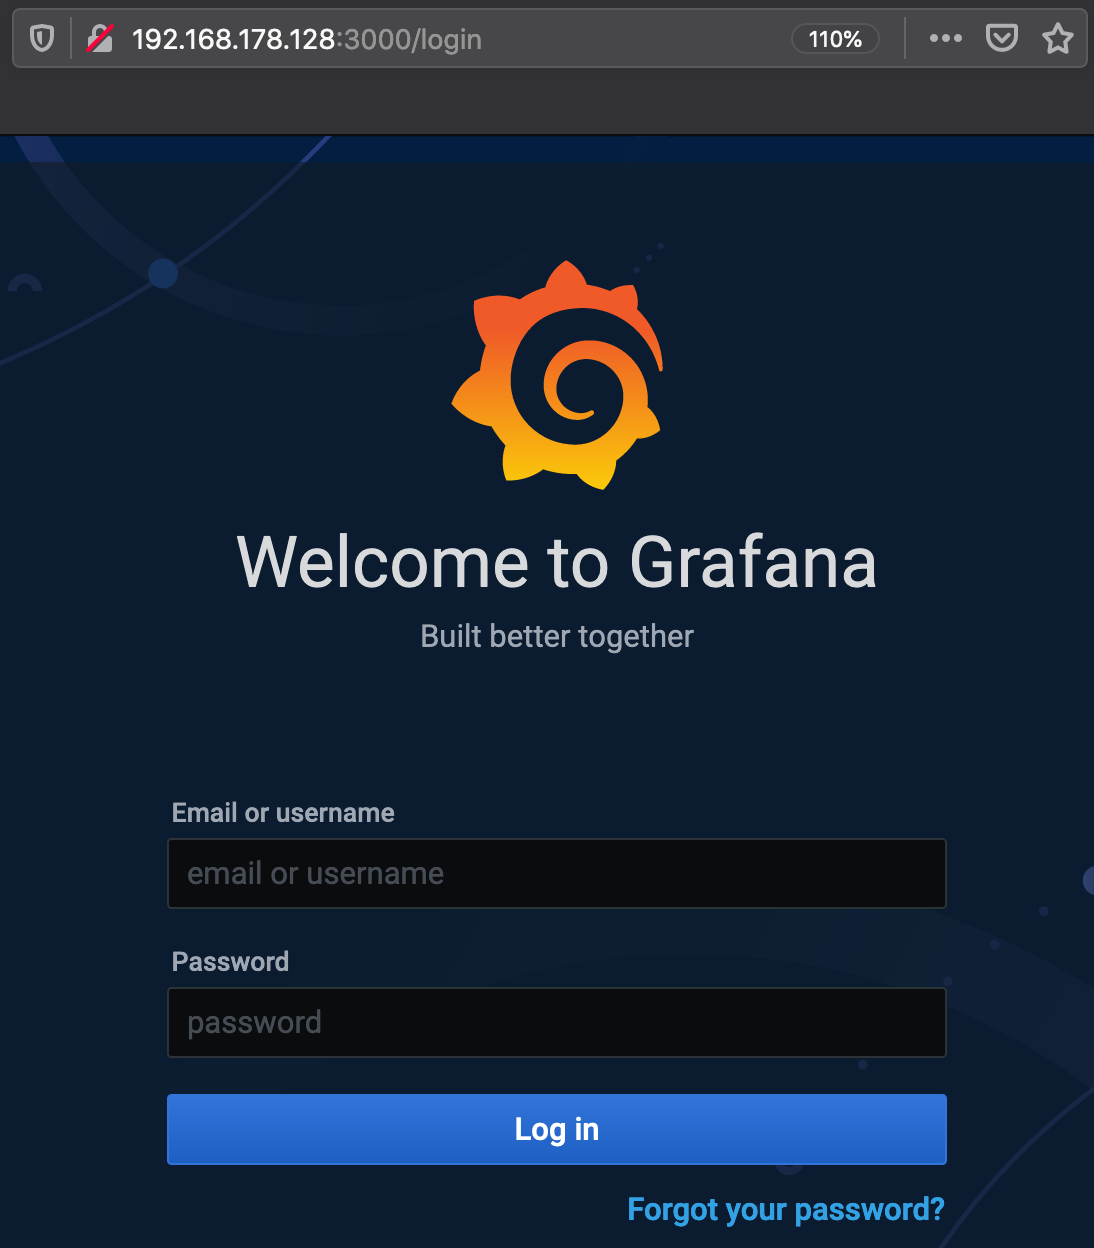
\includegraphics[width=0.6\textwidth]{img/handbuch/grafna_login}
\caption{Grafana Login im Browser}
\label{fig:grafna_login}
\end{figure}
\noindent Im Example Dashboard sind alle Sensordatenplots vorhanden. Wenn weniger Plots benötigt werden oder die Darstellung angepasst werden muss, kann eine Kopie angefertigt und bearbeitet werden.\\
Um Daten im CSV-Format zu exportieren muss zuerst der gewünschte Zeitbereich ausgewählt werden.
Anschließend wird, wie in Abbildung \ref{fig:export_data} zu sehen, im Kontextmenü (Klick auf den Namen eines Plots) unter Inspect die Option Data ausgewählt. 

\begin{figure}[H]
\centering
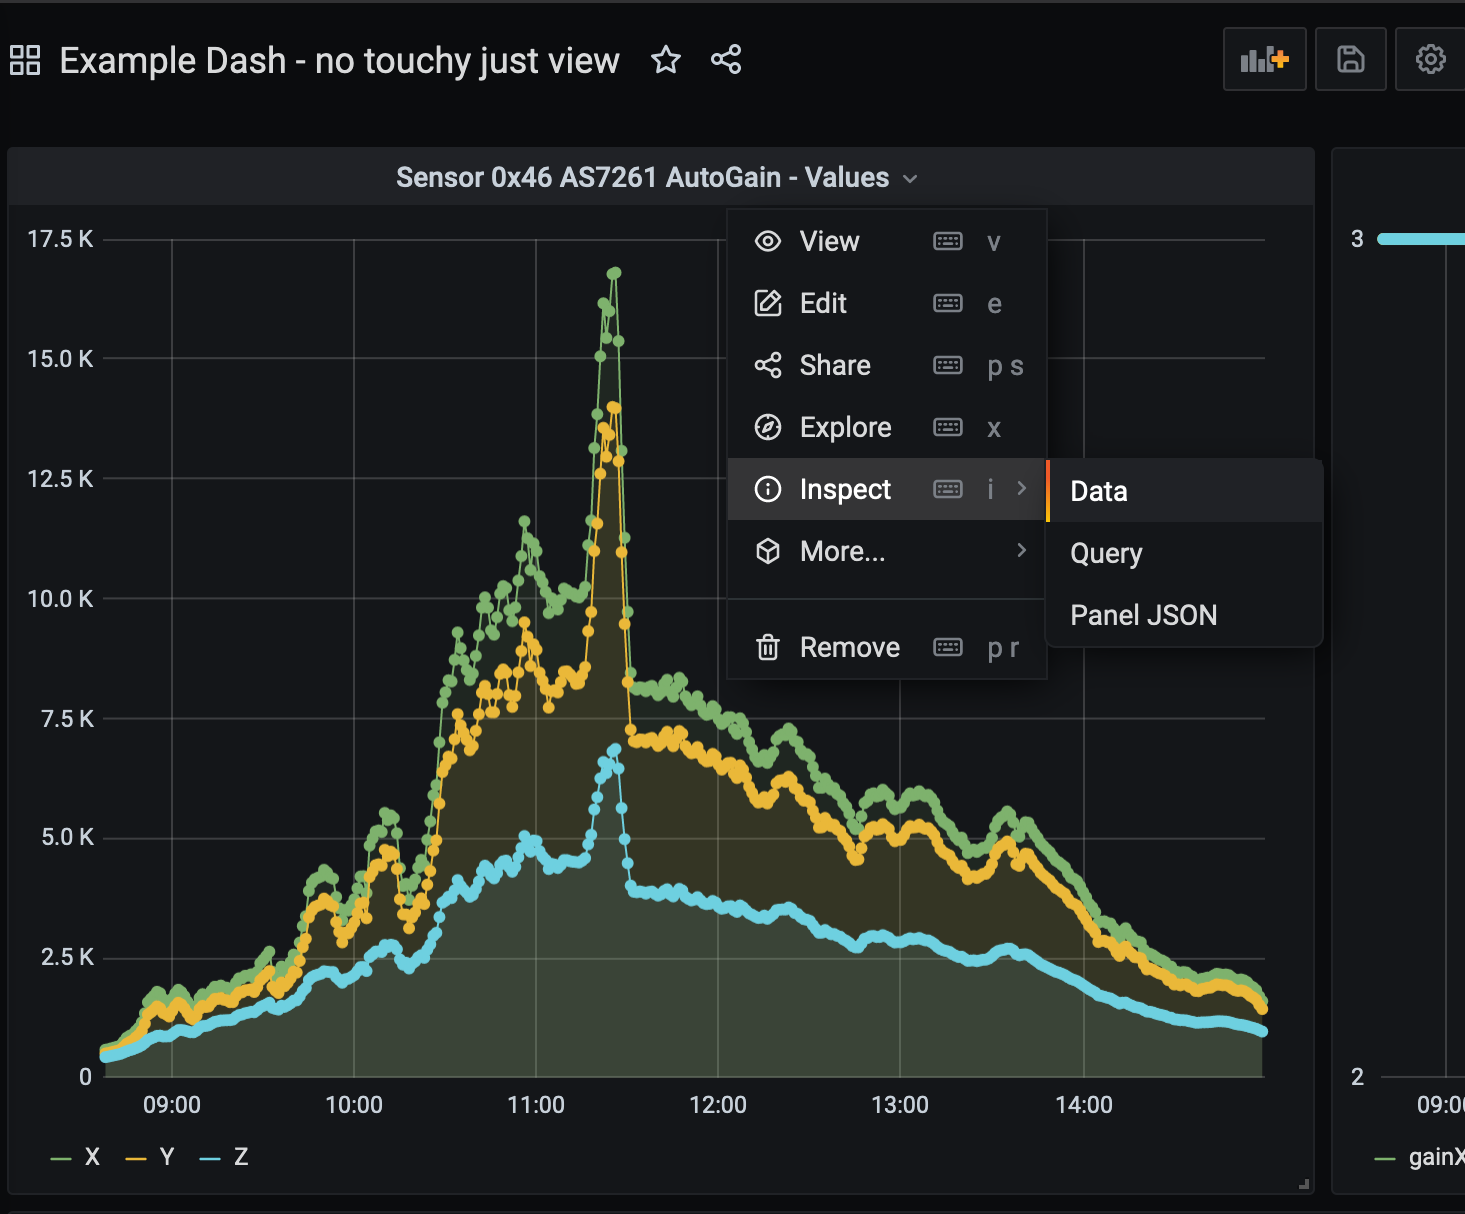
\includegraphics[width=0.6\textwidth]{img/handbuch/Export_Data}
\caption{Screenshot Grafana CSV-Export}
\label{fig:export_data}
\end{figure}
\noindent Daten können nur pro Plot exportiert werden. Um mehr Daten auf einmal zu exportieren, müssen alle gewünschten Daten in einem Plot vereint werden.

\subsection{Messsoftware Beenden/Neustarten}
\label{restart}
Das Programm kann mit Control+C beendet werden.\\
Falls die SSH Verbindung geschlossen wurde, muss diese erst wieder aufgebaut werden.\\
\textbf{ssh pi@[IP-ADRESSE]}\\
Der Screen, in welchem die Messsoftware läuft, muss Attached sein.\\
\textbf{screen -r}\\
Die Liste aktiver Screens kann mit \textbf{screen -list} eingesehen werden.
Weiter Informationen zu Screen: \url{https://linuxize.com/post/how-to-use-linux-screen/}

\noindent Um die Software erneut zu starten, sollte sie wieder neu kompiliert werden, da so immer alle eventuellen Einstellungsänderungen in der Datei default\_values.h übernommen werden:\\
\textbf{cd ~./SpectralSensor}\\
\textbf{screen make}\\




\subsection{IP Adress Scan}
\paragraph{Unter Unix:} sudo nmap -sn 192.168.1.0/24  
\paragraph{Unter Windows:} Mit Hilfe der Software ''PortScan'' \\https://www.the-sz.com/products/portscan/\smallskip

\subsection{Bedeutung der Status LEDs}\label{leds}
\subsubsection{Rapsberry Pi}
Die rote PWR-LED leuchtet kontinuierlich bei stabiler 5V Stromversorgung.\\
Die grüne ACT-LED blinkt, wenn die SD-Karte korrekt arbeitet.
\subsubsection{Status \& Adapterboard}
Die rote Power-LED leuchtet, wenn eine Benutzereingabe zum Starten der Messungen erwartet wird.\\
Die grüne Heartbeat-LED leuchtet, wenn der Messzyklus gestartet wurde, geht aber immer während der eigentlichen Messung aus.
\subsubsection{Sensorboard}
Die roten LEDs D1-AS7261 und D2-AS7265X blinken, wenn es Probleme mit der Firmware auf dem Flaschenspeicher des jeweiligen Sensors gibt.


\subsection{Hilfe}
\textbf{Nach dem Starten der Messung gibt es keine Ausgabe in Terminal:}\\
Vermutlich sind keine Sensoren angeschlossen\\
\textbf{Die Systemzeit ist falsch:}\\
Keiner der NTP-Server aus der Liste /etc/systemd/timesyncd.conf kann erreicht werden.\\
\textbf{Das Webinterface ist nicht erreichbar:}\\
Entweder wurde die Adresse falsch geschrieben oder der Grafana-Server ist abgestürzt / wird nicht mehr automatisch gestartet.\\
\textbf{Error: 500
Write to Database Failed!:}
Der InfluxDB-Server ist abgestürzt / wird nicht mehr automatisch gestartet.
\subsection{Liste Der Verwendeten I2C Adressen \& Translationbytes}
\label{liste_Translationbytes}
Die Translation Bytes (Dezimal) 0- 59 wurden bereits verwendet. Sollten weitere Sensorboards angefertigt werden, muss es hier notiert werden:






